\section{Deferred proofs and implementation details}\label{app:proofs}

This appendix contains only the results needed to support the main paper:
factorization non-identifiability, stable source-center capacity, cross-space
accessibility, the two-sided normalized-thickness result, and the estimators used
in experiments.

\section{Factorization non-identifiability}\label{app:discrepancy}

\subsection{Proof of Theorem~\ref{thm:discrepancy}}

\begin{proof}
Let $(h,p)$ and $(\widetilde h,\widetilde p)$ be admissible pairs satisfying
\[
\widetilde p(\widetilde h(V))=p(h(V))
\]
pathwise. They therefore induce exactly the same projected random variables.
Since $J$ depends on the backbone and projector only through those projected
variables,
\[
J(\widetilde h,\widetilde p)=J(h,p).
\]
If a backbone property takes different values on two admissible factorizations
of the same projected map, the same objective value is compatible with both
values. Hence that property cannot be uniformly certified by the $Z$-only
objective.

The ambiguity is broader than an invertible change of coordinates. An
admissible bijection $\varphi$ gives
\[
\widetilde h=\varphi\circ h,
\qquad
\widetilde p=p\circ\varphi^{-1}.
\]
If a possibly non-injective map $\varphi$ satisfies $p=q\circ\varphi$ on
$\range(h)$, then
\[
\widetilde h=\varphi\circ h,
\qquad
\widetilde p=q
\]
preserves the projected variables while potentially discarding backbone
information. Conversely,
\[
\widetilde h(V)=(h(V),u(V)),
\qquad
\widetilde p(x,y)=p(x)
\]
can append arbitrary backbone information without changing $Z$ or the
objective.
\end{proof}

\begin{corollary}[Projected Gaussianity does not transfer]
\label{cor:gaussian}
Let $Z=(Z_1,Z_2)^\top\sim\mathcal N(0,I_2)$ and define
\[
H=
\begin{pmatrix}
Z_1\\
Z_2+Z_1^2-1
\end{pmatrix},
\qquad
p(h_1,h_2)=
\begin{pmatrix}
h_1\\
h_2-h_1^2+1
\end{pmatrix}.
\]
Then $p(H)=Z$ pathwise, but $H$ is non-Gaussian and
$\Cov(H)=\operatorname{diag}(1,3)$.
\end{corollary}

\begin{proof}
Direct substitution gives $p(H)=Z$. The second coordinate of $H$ contains the
non-Gaussian random variable $Z_1^2-1$. Moreover,
\[
\Var(Z_2+Z_1^2-1)=1+2=3,
\qquad
\Cov(Z_1,Z_2+Z_1^2-1)=0,
\]
so $\Cov(H)=\operatorname{diag}(1,3)$.
\end{proof}

\begin{corollary}[Projected linear separability does not transfer]
\label{cor:separability}
Let $X,R$ be independent Rademacher variables, let $Y=X$, and define
\[
Z=(X,R)^\top,
\qquad
H=(XR,R)^\top,
\qquad
p(h_1,h_2)=(h_1h_2,h_2)^\top.
\]
Then $p(H)=Z$ pathwise. The label is linearly separable in $Z$, whereas the four
support points of $H$ form an XOR configuration and are not linearly separable.
\end{corollary}

\begin{proof}
Because $R^2=1$,
\[
p(H)=(XR^2,R)=(X,R)=Z.
\]
The first coordinate of $Z$ equals $Y$. In $H$, the positive-class points are
$(1,1)$ and $(-1,-1)$, while the negative-class points are $(-1,1)$ and
$(1,-1)$. If an affine score $ah_1+bh_2+c$ strictly separated the classes, the
two positive inequalities would imply $2c>0$, while the two negative
inequalities would imply $2c<0$, a contradiction.
\end{proof}


\section{Stable source-center capacity}\label{app:capacity}

For $S\in\{H,Z\}$, recall
\[
m_s(Q)=\E[S\mid Q],
\qquad
B_s=\Cov(m_s(Q)),
\qquad
A_s=\E[\Cov(S\mid Q)].
\]

\begin{proposition}[Paired views identify stable spread and augmentation thickness]
\label{prop:paired}
Let $S_1,S_2$ be conditionally independent views given $Q$. Then
\[
B_s=\E[(S_1-\mu_s)(S_2-\mu_s)^\top],
\qquad
A_s=\frac12\E[(S_1-S_2)(S_1-S_2)^\top].
\]
\end{proposition}

\begin{proof}
Write $S_i=m_s(Q)+\xi_i$, where $\E[\xi_i\mid Q]=0$. Conditional independence
gives $\E[\xi_1\xi_2^\top\mid Q]=0$, so the cross-covariance of the two views is
$B_s$. Also $S_1-S_2=\xi_1-\xi_2$; the two conditional residual covariances add
and the cross terms vanish, giving the second identity.
\end{proof}

\begin{proposition}[Pooled centers suppress augmentation variation]
\label{prop:finite-centers}
Let $S^{(1)},\ldots,S^{(V)}$ be conditionally independent views given $Q$ and
\[
\overline S_V=\frac1V\sum_{v=1}^V S^{(v)}.
\]
Then
\[
\E[\overline S_V]=\mu_s,
\qquad
\Cov(\overline S_V)=B_s+\frac1V A_s.
\]
\end{proposition}

\begin{proof}
Write
\[
\overline S_V=m_s(Q)+\overline\xi_V,
\qquad
\overline\xi_V=\frac1V\sum_{v=1}^V\xi^{(v)}.
\]
The law of total covariance gives
\[
\Cov(\overline S_V)
=
B_s+\E[\Cov(\overline\xi_V\mid Q)].
\]
Conditional independence gives
$\E[\Cov(\overline\xi_V\mid Q)]=A_s/V$.
\end{proof}

\begin{proof}[Proof of Proposition~\ref{prop:capacity-main}]
Equation~\eqref{eq:pooled-cov-main} gives
\[
I_d=B_s+\frac1V A_s,
\qquad
B_s=I_d-\frac1V A_s.
\]
Since $0\preceq A_s\preceq\alpha I_d$,
\[
\left(1-\frac{\alpha}{V}\right)I_d
\preceq B_s\preceq I_d.
\]
Therefore
\[
\tr B_s\ge d\left(1-\frac{\alpha}{V}\right),
\qquad
\norm{B_s}_{\rm op}\le1,
\]
which yields
\[
\srank(B_s)\ge d\left(1-\frac{\alpha}{V}\right).
\]
\end{proof}

The exact-whitening statement in the main paper is the cleanest special case.
For completeness, the same conclusion survives finite moment loss.

\begin{theorem}[Finite-loss pooled-center control]\label{thm:kl}
Let
\[
\widetilde B_V=B+\frac1V A,
\qquad
A\succeq0,
\]
on a $d$-dimensional active subspace. If
\[
\cK_{\rm ctr}(\mu,\widetilde B_V)\le\varepsilon,
\]
then $\norm{\mu}^2\le2\varepsilon$ and every eigenvalue of
$\widetilde B_V$ lies in $[\ell_\varepsilon,u_\varepsilon]$, where
$\ell_\varepsilon\le1\le u_\varepsilon$ are the two solutions of
\[
x-\log x-1=2\varepsilon.
\]
If additionally $\norm{A}_{\rm op}\le\alpha<V\ell_\varepsilon$, then
\[
\left(\ell_\varepsilon-\frac{\alpha}{V}\right)I_d
\preceq B\preceq u_\varepsilon I_d
\]
and
\[
\srank(B)
\ge
d\,\frac{\ell_\varepsilon-\alpha/V}{u_\varepsilon}.
\]
\end{theorem}

\begin{proof}
Let $\widetilde\lambda_1,\ldots,\widetilde\lambda_d$ be the eigenvalues of
$\widetilde B_V$. Then
\[
2\cK_{\rm ctr}(\mu,\widetilde B_V)
=
\norm{\mu}^2+
\sum_{j=1}^d
\left(\widetilde\lambda_j-\log\widetilde\lambda_j-1\right).
\]
The scalar function $f(x)=x-\log x-1$ is nonnegative and vanishes only at
$x=1$. Hence the loss bound implies $\norm{\mu}^2\le2\varepsilon$ and
\[
\ell_\varepsilon I_d
\preceq\widetilde B_V
\preceq u_\varepsilon I_d.
\]
Since $B=\widetilde B_V-A/V$ and
$0\preceq A\preceq\alpha I_d$,
\[
\left(\ell_\varepsilon-\frac{\alpha}{V}\right)I_d
\preceq B\preceq u_\varepsilon I_d.
\]
The stated stable-rank bound follows by lower-bounding $\tr B$ and
upper-bounding $\norm{B}_{\rm op}$.
\end{proof}


\section{Cross-space accessibility}\label{app:accessibility}

Here we record the least-squares identities behind the accessibility diagnostic
used in the main paper. Let
\[
W_c
=
\argmin_W
\E\norm{
\overline m_z(Q)-W(m_h(Q)-\mu_h)
}^2
\]
and
\[
e_c(Q)
=
\overline m_z(Q)-W_c(m_h(Q)-\mu_h),
\qquad
\Sigma_c=\Cov(e_c).
\]
Projected source centers are whitened so that
$\Cov(\overline m_z)=I_{r_z}$.

Population least-squares orthogonality immediately gives
\begin{equation}\label{eq:access-cov-decomp-app}
I_{r_z}
=
W_cB_hW_c^\top+\Sigma_c.
\end{equation}
Taking traces yields
\[
R^2_{\rm acc}
=
1-\frac{\tr\Sigma_c}{r_z}
=
\frac{\tr(W_cB_hW_c^\top)}{r_z}.
\]
For any projected direction $u\in\R^{r_z}$,
\begin{equation}\label{eq:directional-access-app}
\min_a
\E\left[
\left(
u^\top\overline m_z(Q)
-
a^\top(m_h(Q)-\mu_h)
\right)^2
\right]
=
u^\top\Sigma_cu.
\end{equation}

To prove the organization-transfer statement in
\eqref{eq:organization-transfer}, let
\[
P_{\cM_z}y=u_y^\top\overline m_z(Q).
\]
The candidate
$u_y^\top W_c(m_h(Q)-\mu_h)$ belongs to $\cM_h$, so
\[
\begin{aligned}
d_h(y)
&\le
\norm{y-P_{\cM_z}y}_{L^2}
+
\norm{u_y^\top e_c}_{L^2}\\
&=
d_z(y)+\sqrt{u_y^\top\Sigma_cu_y}.
\end{aligned}
\]

\paragraph{Average versus worst-direction accessibility.}
If $R^2_{\rm acc}\ge1-\delta$, then
$\tr\Sigma_c\le r_z\delta$. Therefore, for any $\tau>0$,
\[
\#\{j:\lambda_j(\Sigma_c)>\tau\}
\le
\frac{r_z\delta}{\tau}.
\]
Thus a high average score controls most center-whitened projected directions,
but it need not control the worst direction. When the stronger condition
$\norm{\Sigma_c}_{\rm op}\le\varepsilon_c^2$ holds, every normalized
$g\in\cM_z$ lies within $L^2$ distance $\varepsilon_c$ of $\cM_h$; this is the
usual largest-principal-angle interpretation of the two center subspaces
\citep{stewart2016cs}.


\section{Normalized augmentation thickness}\label{app:resolution}

This section proves Theorem~\ref{thm:retained-resolution}. Recall
\[
\Theta_h
=
B_h^{\dagger/2}A_hB_h^{\dagger/2}.
\]
On the active center subspace, write the whitened representation as
\[
\overline H
=
\overline m_h(Q)+\xi_h,
\qquad
\Cov(\overline m_h)=I_{r_h},
\qquad
\E[\xi_h\mid Q]=0,
\qquad
\Cov(\xi_h)=\Theta_h,
\]
and for a centered source target $y$ recall
\[
\cE_{\mathsf A}(y)
=
\min_f\E[(y(Q)-f(V))^2],
\]
where the minimum ranges over square-integrable functions of a single augmented view.

\subsection{Reading direction and center error}

Let $P_{\cM_h}y=a^\top\overline m_h(Q)$ and write
\[
y=a^\top\overline m_h(Q)+r,
\qquad
r\perp\cM_h,
\qquad
\norm{r}_{L^2}=d_h(y).
\]
Because the coordinates of $\overline m_h$ are orthonormal in $L^2$,
$\norm{a}^2=\norm{P_{\cM_h}y}^2=\norm{y}^2-d_h(y)^2$. The thickness along the reading
direction is
\[
\lambda_h(a)=\frac{a^\top\Theta_ha}{\norm{a}^2}.
\]
In the original coordinates the center reader is $u=B_h^{\dagger/2}a$ and
$a^\top\Theta_ha/\norm{a}^2=u^\top A_hu/u^\top B_hu$, the per-direction quantity of
Section~\ref{sec:thickness}.

\subsection{One identity}

Since $\E[\overline H-\overline m_h(Q)\mid Q]=0$ and $r$ is a function of $Q$, the residual
$r$ is uncorrelated with every linear function of $\overline H$. For any linear predictor
$u^\top\overline H$,
\[
\E[(y-u^\top\overline H)^2]
=
\norm{r}^2
+
\E\big[(a^\top\overline m_h(Q)-u^\top\overline H)^2\big].
\]
The second term is the error of predicting the center coordinate $a^\top\overline m_h$ from
$\overline H$. Because
\[
\Cov(\overline H)=I_{r_h}+\Theta_h,
\qquad
\Cov(\overline H,\overline m_h)=I_{r_h},
\]
population least squares gives the residual covariance
\[
I_{r_h}-(I_{r_h}+\Theta_h)^{-1}
=
\Theta_h(I_{r_h}+\Theta_h)^{-1},
\]
so the optimal linear single-view read costs
\[
\inf_u\E[(y-u^\top\overline H)^2]
=
d_h(y)^2+a^\top\Theta_h(I_{r_h}+\Theta_h)^{-1}a.
\]
The center reader $u=a$ is one admissible predictor, with
$\E[(y-a^\top\overline H)^2]=d_h(y)^2+a^\top\Theta_ha=d_h(y)^2+\norm{a}^2\lambda_h(a)$
by the same orthogonality; equivalently $\Theta_h(I+\Theta_h)^{-1}\preceq\Theta_h$. This
proves part (i).

\subsection{Too little retained thickness}

Every linear function of $\overline H$ is a square-integrable function of the single view
$V$, hence an admissible predictor in the definition of $\cE_{\mathsf A}(y)$. By part (i),
\[
\cE_{\mathsf A}(y)
\le
\inf_u\E[(y-u^\top\overline H)^2]
=
d_h(y)^2+a^\top\Theta_h(I+\Theta_h)^{-1}a
\le
d_h(y)^2+\norm{a}^2\lambda_h(a)
\le
d_h(y)^2+\lambda_h(a),
\]
using $\norm{a}^2\le\norm{y}^2\le1$ in the last step. Rearranging gives
\eqref{eq:too-thin-main}, and substituting $\norm{a}^2=\norm{y}^2-d_h(y)^2$ gives the
threshold form: whenever $\cE_{\mathsf A}(y)>d_h(y)^2$,
\[
\lambda_h(a)\ge\frac{\cE_{\mathsf A}(y)-d_h(y)^2}{\norm{y}^2-d_h(y)^2}.
\]
The bound is attained exactly when the optimal linear single-view read of $\overline H$
is the Bayes predictor of $y$ from a view.

For the worst-direction form, $\lambda_h(a)\le\norm{\Theta_h}_{\rm op}$ because
$\lambda_h(a)$ is a Rayleigh quotient of $\Theta_h$, and for $0\le\lambda\le\cE$,
$\cE-\lambda-(\sqrt{\cE}-\sqrt{\lambda})^2=2\sqrt{\lambda}(\sqrt{\cE}-\sqrt{\lambda})\ge0$.
Hence $d_h(y)^2\ge\cE_{\mathsf A}(y)-\norm{\Theta_h}_{\rm op}\ge(\sqrt{\cE_{\mathsf A}(y)}-\sqrt{\norm{\Theta_h}_{\rm op}})_+^2$,
which is the earlier statement; it discards the direction and is never tighter. This
proves part (ii).

\subsection{Too much retained thickness}

Finally,
\[
X\mapsto X(I+X)^{-1}=I-(I+X)^{-1}
\]
is operator monotone increasing on positive-semidefinite matrices, so for fixed center
organization and reading direction the second term of
\eqref{eq:organization-thickness-decomp} is monotone nondecreasing in $\Theta_h$. This
proves part (iii) of Theorem~\ref{thm:retained-resolution}.

\section{Estimation and implementation details}\label{app:experiments}

\subsection{Pooled-center covariance during training}

For a training batch containing $B$ source objects and $V$ independently
augmented views of each object, compute
\[
\widehat m_{s,i}
=
\frac1V\sum_{v=1}^V S_{iv},
\qquad
\widehat\mu_s
=
\frac1B\sum_{i=1}^B\widehat m_{s,i},
\]
and
\[
\widehat B_{s,V}^{\rm batch}
=
\frac1{B-1}
\sum_{i=1}^B
(\widehat m_{s,i}-\widehat\mu_s)
(\widehat m_{s,i}-\widehat\mu_s)^\top.
\]
With the unbiased $1/(B-1)$ normalization,
\[
\E[\widehat B_{s,V}^{\rm batch}]
=
B_s+\frac1V A_s.
\]
If the implementation uses $1/B$, the expectation receives the usual factor
$(B-1)/B$; this is separate from the finite-view correction $A_s/V$.

The population guarantees concern the pooled population covariance rather than a
single raw batch covariance. In particular, a raw covariance is rank deficient
when the number of centered source samples is smaller than its dimension.

\subsection{Random orthonormal slices and covariance stabilization}

For high-dimensional representations, the moment penalty can be applied to a
random row-orthonormal slice
\[
R\in\R^{k\times d},
\qquad
RR^\top=I_k.
\]
Fresh slices reduce covariance cost while exposing different directions over
training.

\begin{theorem}[Expectation guarantee for random orthonormal slices]
\label{thm:random-slices}
Let $R\in\R^{k\times d}$ be Haar-uniform subject to $RR^\top=I_k$. Then
\[
\E_R\norm{R\mu}^2
=
\frac{k}{d}\norm{\mu}^2.
\]
For any symmetric $A\in\R^{d\times d}$,
\[
\E_R\norm{RAR^\top}_{\rm F}^2=0
\quad\Longleftrightarrow\quad
A=0.
\]
\end{theorem}

\begin{proof}
Let $P=R^\top R$. Rotational symmetry gives
$\E_RP=(k/d)I_d$, proving the first identity. If $A\ne0$, some unit vector $u$
satisfies $u^\top Au\ne0$. Any slice whose row space contains $u$ has
$RAR^\top\ne0$, and by continuity this remains true on a positive-measure set of
slices. Hence the expected nonnegative sliced covariance error is positive.
\end{proof}

A fixed slice can of course miss errors in its kernel, so the guarantee is in
expectation over fresh slices rather than an equivalence between one sliced
objective and the full covariance objective. When the sketched covariance is
poorly estimated, we use shrinkage or a running covariance accumulated across
steps, with gradients only through the current batch.

\subsection{Estimating $B_s$, $A_s$, and $\Theta_s$}

From conditionally independent paired views $(S_{1i},S_{2i})$, estimate
\[
\widehat\mu_s
=
\frac1{2n}\sum_{i=1}^n(S_{1i}+S_{2i}),
\]
\[
\widehat A_s
=
\frac1{2n}\sum_{i=1}^n
(S_{1i}-S_{2i})(S_{1i}-S_{2i})^\top,
\]
and
\[
\widehat B_s
=
\frac1{2n}\sum_{i=1}^n
\left[
(S_{1i}-\widehat\mu_s)(S_{2i}-\widehat\mu_s)^\top
+
(S_{2i}-\widehat\mu_s)(S_{1i}-\widehat\mu_s)^\top
\right].
\]
The $A_s$ estimator is unbiased. The plug-in $B_s$ estimator is consistent but
not exactly unbiased because the same observations estimate the mean, and it may
be indefinite at finite sample size. We report the raw symmetrized estimate and
use a separately identified PSD-regularized version only when inversion is
required.

An evaluation-only alternative removes the finite-view term explicitly. Split
the views of each source into two conditionally independent groups, form group
means $\overline S_i^{(a)}$ and $\overline S_i^{(b)}$, and use
\[
\Cov(\overline S^{(a)},\overline S^{(b)})=B_s.
\]
The finite-sample cross-covariance need not be positive semidefinite, so this is
a diagnostic rather than the default log-det training covariance.

We form
\[
\widehat\Theta_s
=
\widehat B_s^{\dagger/2}
\widehat A_s
\widehat B_s^{\dagger/2}
\]
only on an eigenvalue-truncated support of $\widehat B_s$. The truncation
threshold and effective rank are reported with the measurement. Varying the
number of pooled views provides a direct empirical check of
\[
\widehat B_{s,V}
\approx
\widehat B_s+\frac1V\widehat A_s.
\]

\subsection{Estimating cross-space accessibility}

Estimate source centers from multiple held-out views, split by source object,
whiten the $Z$ centers, and fit a multi-output linear map from $H$ centers to
$Z$ centers. The primary summary is
\[
\widehat R^2_{\rm acc}
=
1-\frac{\tr\widehat\Sigma_c}{r_z},
\qquad
\widehat\Sigma_c
=
\widehat\Cov(e_c).
\]
We additionally report directional residuals
\[
\widehat u^\top\widehat\Sigma_c\widehat u
\]
when a projected direction is of interest. The residual spectrum can be used to
distinguish a high average accessibility score from a small number of poorly
accessible directions.

Finite-view center estimates create an errors-in-variables effect. We therefore
vary the number of views per source or account for center-estimation noise when
interpreting accessibility values.

For task-aligned organization diagnostics, estimate $d_z(y)$ and $d_h(y)$ from
held-out source centers. If
$\widehat u_y^\top\widehat{\overline m}_z$ is the projected component of the
task, compare the observed backbone organization error with
\[
d_z(y)
+
\sqrt{
\widehat u_y^\top
\widehat\Sigma_c
\widehat u_y
},
\]
the empirical counterpart of \eqref{eq:organization-transfer}.


\section{Treatment effects across SSL methods}\label{app:treatment-zoo}

\begin{figure}[p]
  \centering
  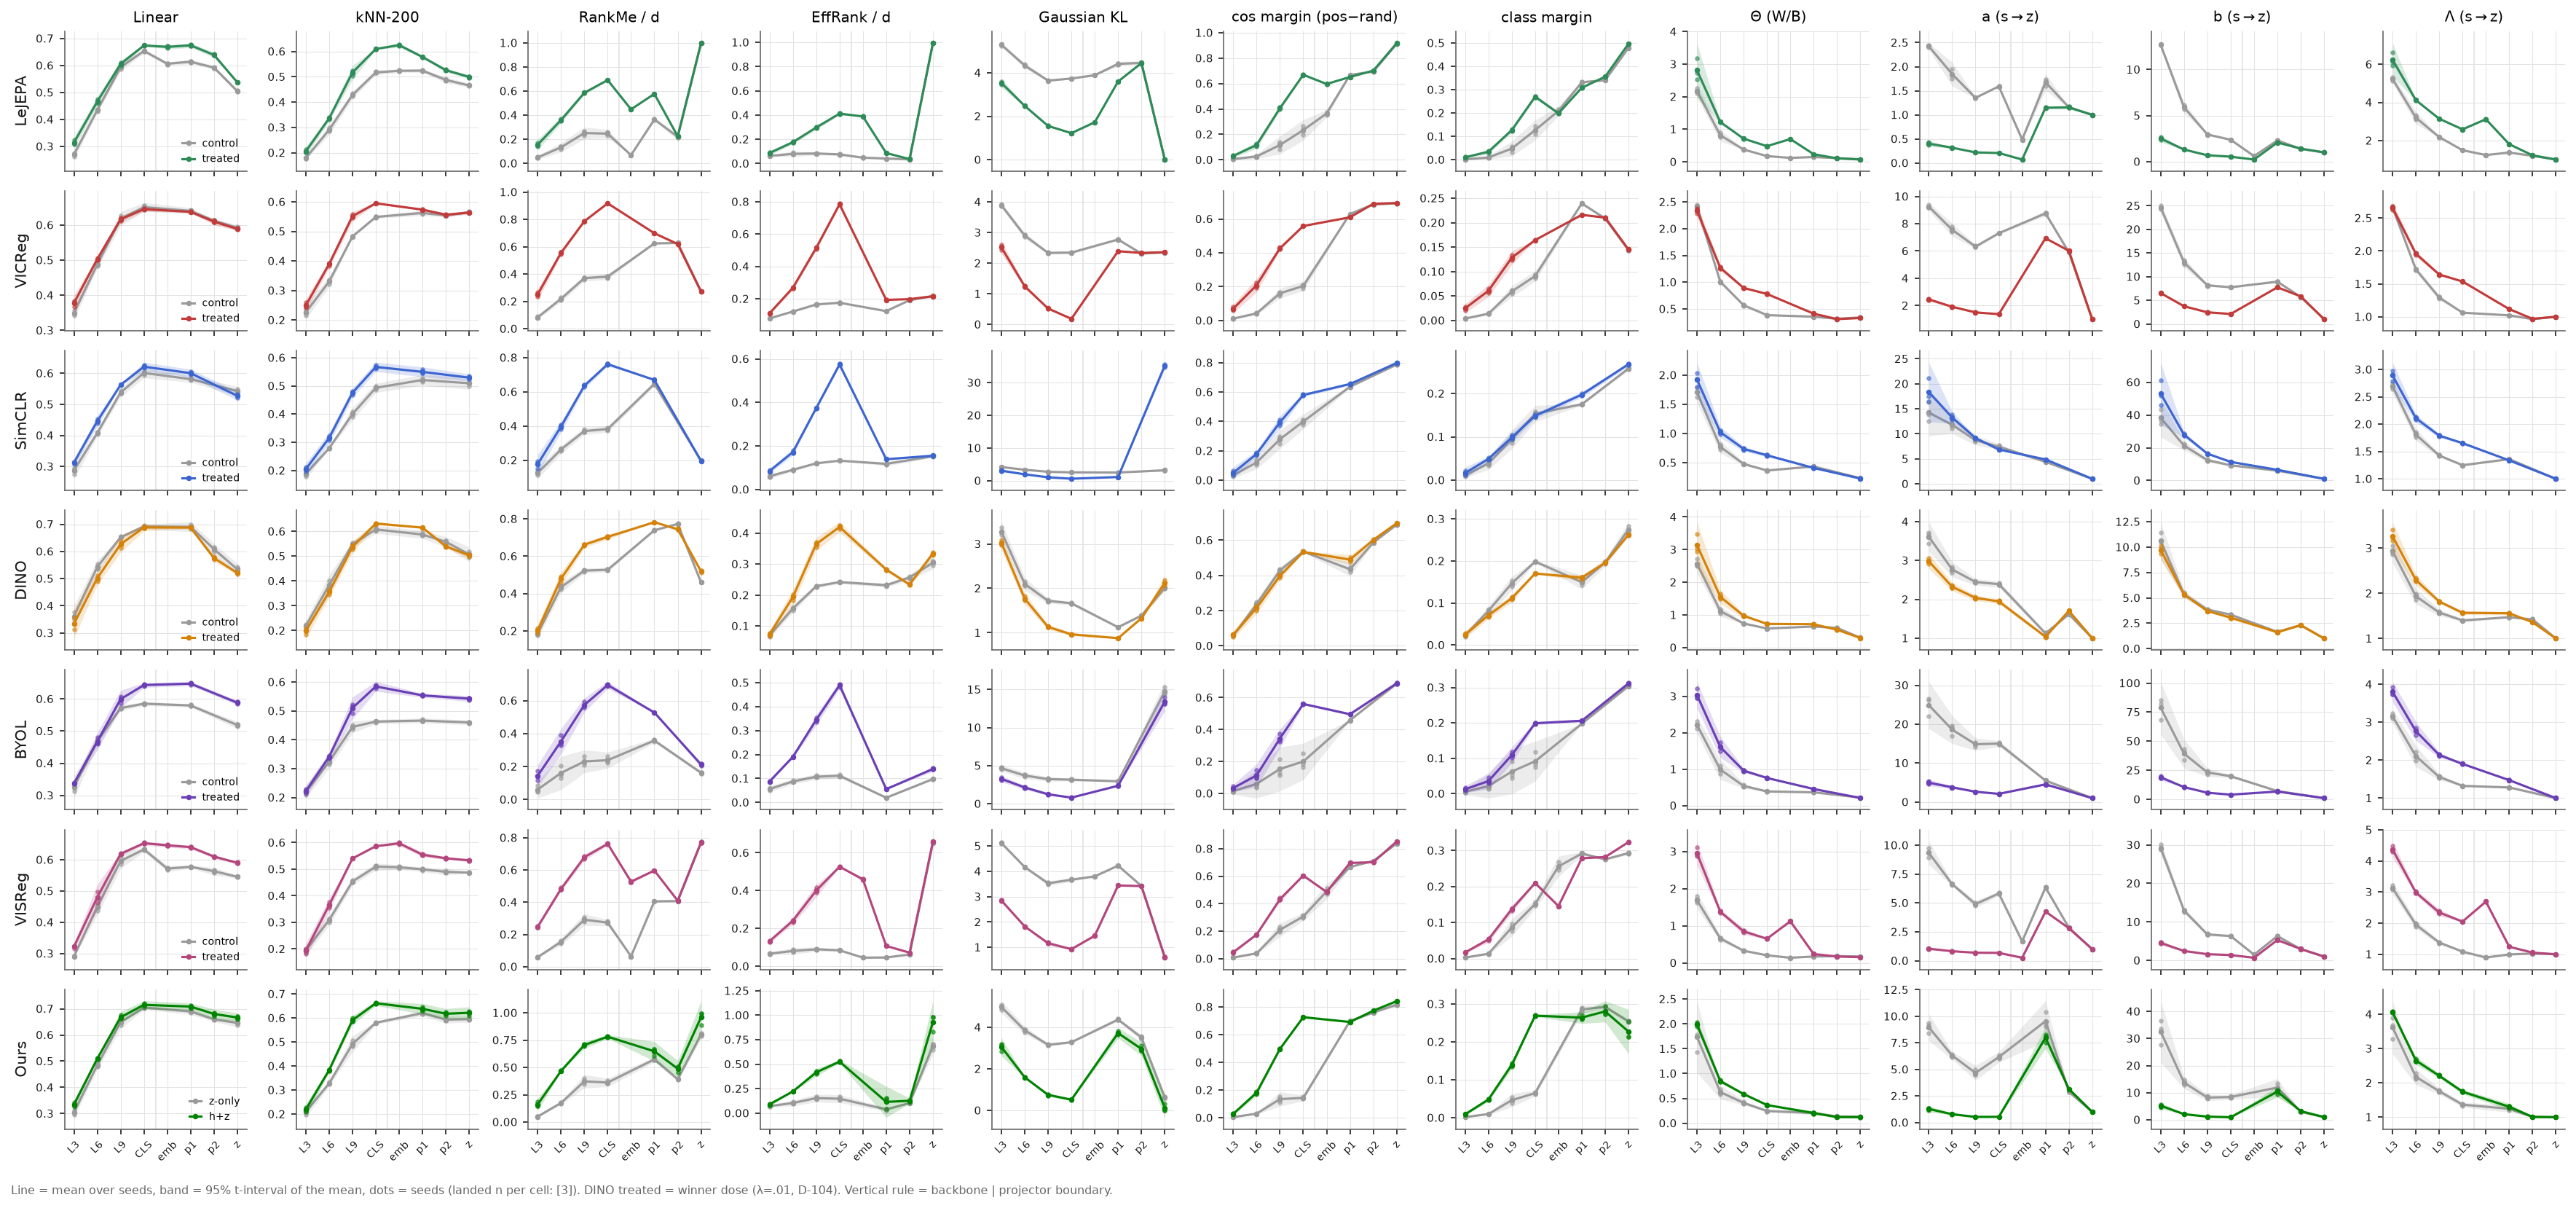
\includegraphics[width=\linewidth]{figures/fig_treatment_appendix.png}
  \caption{Full treatment comparison across methods and reported representation
  metrics. Main-text figures show the quantities most directly used in the
  argument.}
  \label{fig:treatment-appendix}
\end{figure}
